\Class{Psion}
{Resist all you like. I have ways of making you think.}{Dechares, Dwarven inquisitor}

The psion learns the Way, a philosophy of mental discipline, to become master of his will, or innate mental power. Most aspiring psions seek out an instructor, a master of the Way. Most Athasian cities contain psionic academies where students receive instructions in exchange for money or loyal service.

\PsychicTable{The Psion}{
1st  & +0         & +0 & +0 & +2  & Bonus feat, discipline & 20 & 3  & 1 \\
2nd  & +1         & +0 & +0 & +3  &                        & 25 & 5  & 2 \\
3rd  & +2         & +1 & +1 & +3  &                        & 30 & 7  & 2 \\
4th  & +3         & +1 & +1 & +4  &                        & 35 & 9  & 2 \\
5th  & +3         & +1 & +1 & +4  & Bonus feat             & 40 & 10 & 2 \\
6th  & +4         & +2 & +2 & +5  &                        & 45 & 11 & 3 \\
7th  & +5         & +2 & +2 & +5  &                        & 50 & 12 & 3 \\
8th  & +6/+1      & +2 & +2 & +6  &                        & 55 & 13 & 3 \\
9th  & +6/+1      & +3 & +3 & +6  &                        & 60 & 14 & 3 \\
10th & +7/+2      & +3 & +3 & +7  & Bonus feat             & 62 & 15 & 4 \\
11th & +8/+3      & +3 & +3 & +7  &                        & 64 & 16 & 4 \\
12th & +9/+4      & +4 & +4 & +8  &                        & 68 & 17 & 4 \\
13th & +9/+4      & +4 & +4 & +8  &                        & 70 & 18 & 4 \\
14th & +10/+5     & +4 & +4 & +9  &                        & 72 & 19 & 5 \\
15th & +11/+6/+1  & +5 & +5 & +9  & Bonus feat             & 74 & 20 & 5 \\
16th & +12/+7/+2  & +5 & +5 & +10 &                        & 76 & 21 & 5 \\
17th & +12/+7/+2  & +5 & +5 & +10 &                        & 78 & 22 & 5 \\
18th & +13/+8/+3  & +6 & +6 & +11 &                        & 80 & 23 & 6 \\
19th & +14/+9/+4  & +6 & +6 & +11 &                        & 82 & 24 & 6 \\
20th & +15/+10/+5 & +6 & +6 & +12 & Bonus feat             & 84 & 25 & 6 \\
}

\begin{figure}[t!]
\centering
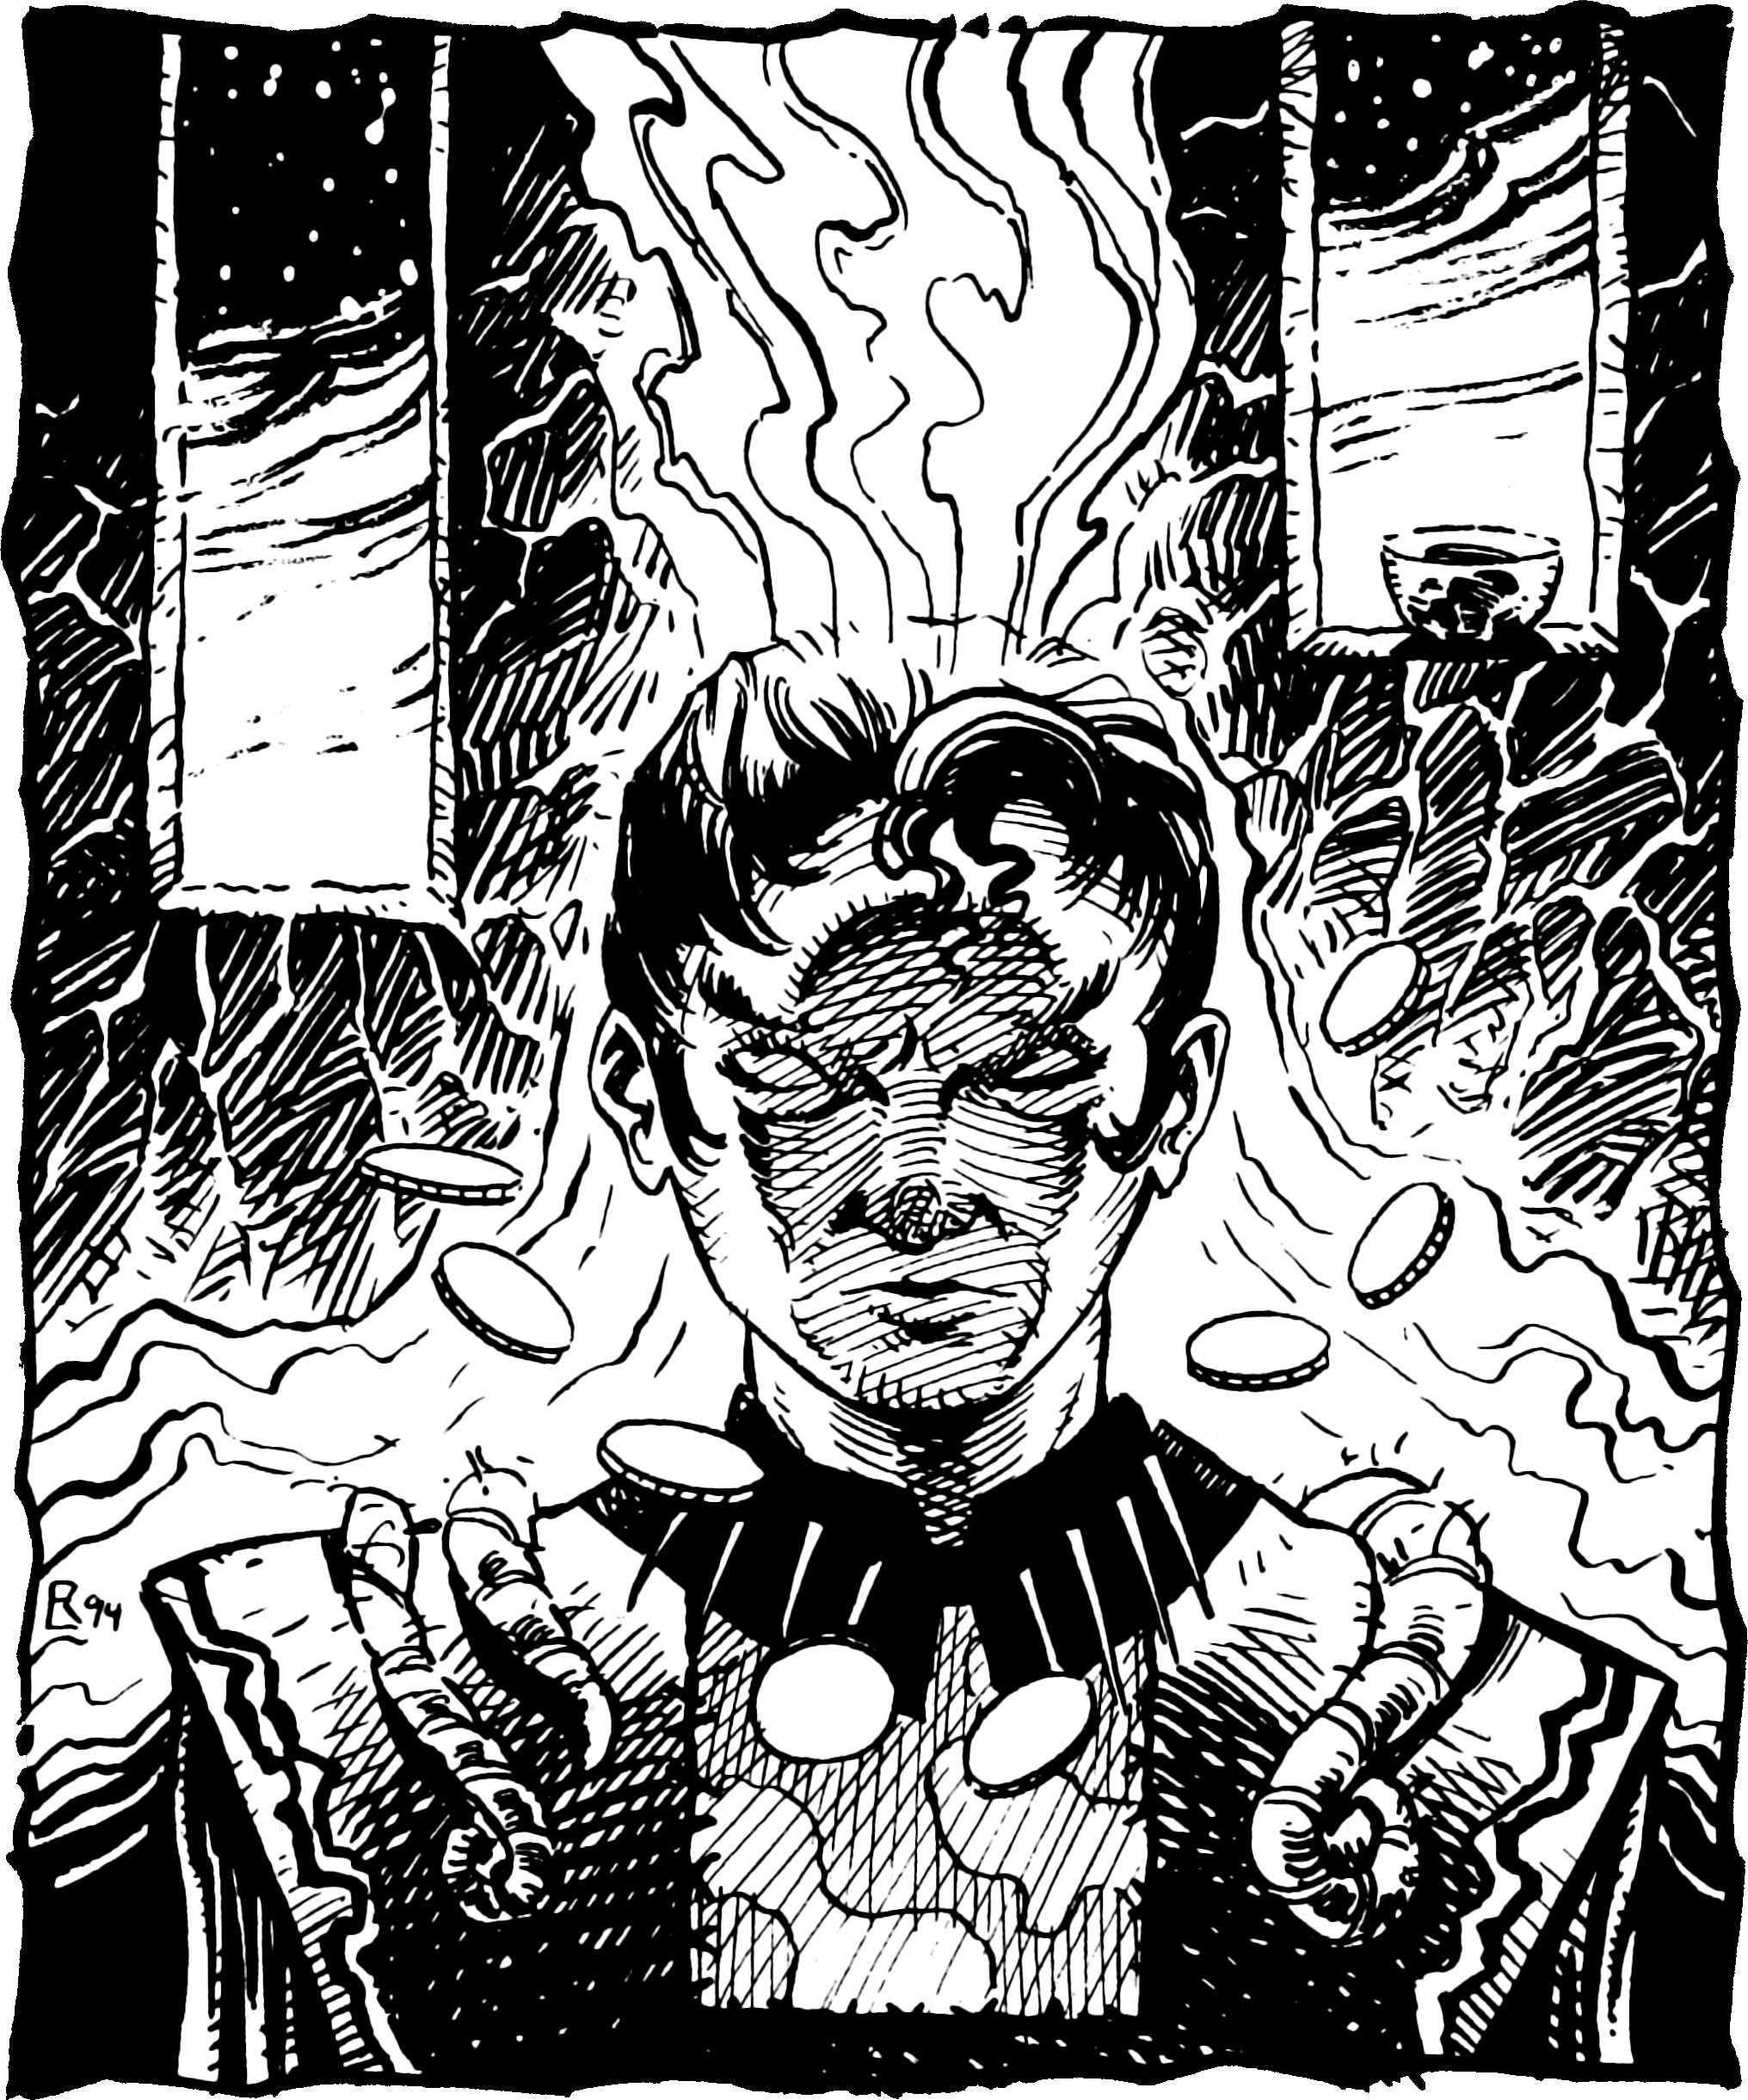
\includegraphics[width=\columnwidth]{images/psion-2.png}
\WOTC
\end{figure}

\subsection{Making a Psion}
The psion learns the Way in order to shape his Will. The psion uses, through study called the Way, how to manifest the power inherent in his inner self. The psion is able to project this power, the Will, into creating all sorts of supernatural effects. The psion may know a limited number of ways to shape his will, but he enjoys great flexibility in how he uses his known powers.

\textbf{Races:} Nearly all living creatures have a latent psionic capacity, and psions are found among all sentient races of the Tablelands, and even among some creatures that are not ordinarily considered sentient.

\textbf{Alignment:} The search for refinement of the Way tends to draw many psions into a neutral view of the world, so most psions have one part of their alignment that is neutral. Good psions may spend their time in search of new powers, or help their village defend itself against predators, or maybe join the ranks of Merchant Houses. Evil psions may serve as agents in service of the sorcerer-kings, or as more shady agents of Merchant Houses, or simply work as mercenaries and offer their specialized services to the highest bidder. Even though many psions tend to have a neutral view of the world, they can be of any alignment.

\subsection{Game Rule Information}

\textbf{Hit Die:} d6.

\subsubsection{Class Skills}

\skill{Autohypnosis} (Wis), \skill{Concentration} (Con), \skill{Craft} (Int), \skill{Handle Animal} (Cha), \skill{Knowledge} (nobility and royalty) (Int), \skill{Knowledge} (psionics) (Int), \skill{Perform} (Cha), \skill{Profession} (Wis), \skill{Psicraft} (Int), Speak Language (N/A), and \skill{Use Rope} (Dex).

\textbf{Skill Points per Level:} 2 + Int modifier ($\times 4$ at 1st level).

\subsubsection{Class Features}

\textbf{Weapon and Armor Proficiency:} Psions are proficient with the club, dagger, heavy crossbow, light crossbow, quarterstaff, and shortspear. They are not proficient with any type of armor or shield. Armor does not, however, interfere with the manifestation of powers.

\textbf{Power Points per Day:} A psion's ability to manifest powers is limited by the power points he has available. His base daily allotment of power points is given on \tabref{The Psion}. In addition, he receives bonus power points per day if he has a high ability score (see \tabref{Ability Scores and Bonus Power Points}). A psion gain bonus power points with Constitution, Intelligence, and Wisdom. His race may also provide bonus power points per day, as may certain feats and items.

\textbf{Discipline:} Every psion must decide at 1st level which psionic discipline he will specialize in. Choosing a discipline provides a psion with access to the powers restricted to that discipline. However, choosing a discipline also means that the psion cannot learn powers that are restricted to other disciplines. He can't even use such powers by employing psionic items.

Beginning at 2nd level and every four levels thereafter, the psion gains access to a new discipline and may learn powers of this new discipline.

\textbf{Powers Known:} A psion begins play knowing three psion powers of your choice. Each time he achieves a new level, he unlocks the knowledge of new powers.

Choose the powers known from the list of powers of your chosen discipline. You cannot choose powers from discipline lists other than your own discipline list. You must fulfill the power prerequisites (if any) to learn a power---these are powers that you must know before learning that power.

The number of times a psion can manifest powers in a day is limited only by his daily power points.

A psion simply knows his powers; they are ingrained in his mind. He does not need to prepare them (in the way that some spellcasters prepare their spells), though he must get a good night's sleep each day to regain all his spent power points.

The Difficulty Class for saving throws against psion powers is 10 + the power's level + the psion's key ability modifier. The key ability depends on the discipline of the power being manifested. See \tabref{Disciplines and Associated Abilities}.

\Table{Disciplines and Associated Abilities}{XX}{
\tableheader Discipline & \tableheader Associated Ability \\
Psychometabolism & Constitution \\
Psychoportation  & Constitution \\
Psychokinesis    & Intelligence \\
Metacreativity   & Intelligence \\
Clairscience     & Wisdom \\
Telepathy        & Wisdom \\
}

\textbf{Maximum Power Level Known:} A psion begins play with the ability to learn 1st-level powers. As he attains higher levels, a psion may gain the ability to master more complex powers.

To learn or manifest a power, a psion must have a key ability score of at least 10 + the power's level. The key ability depends on the discipline of the power. See \tabref{Disciplines and Associated Abilities}.

\textbf{Bonus Feats:} A psion gains a bonus feat at 1st level, 5th level, 10th level, 15th level, and 20th level. This feat must be a psionic feat, a metapsionic feat, or a psionic item creation feat.

These bonus feats are in addition to the feats that a character of any class gains every three levels. A psion is not limited to psionic feats, metapsionic feats, and psionic item creation feats when choosing these other feats.

\subsubsection{Psionic Disciplines}
A discipline is one of six groupings of powers, each defined by a common theme. The six disciplines are clairsentience, metacreativity, psychokinesis, psychometabolism, psychoportation, and telepathy.

\textbf{Clairsentience:} A psion who chooses clairsentience is known as a seer. Seers can learn precognitive powers to aid their comrades in combat, as well as powers that permit them to gather information in many different ways.

\textbf{Metacreativity:} A psion specializing in metacreativity is known as a shaper. This discipline include powers that combine of two other disciplines, and powers that deal with psionics itself. %includes powers that draw ectoplasm or matter from the Astral Plane, creating semisolid and solid items such as armor, weapons, or animated constructs to do battle at the shaper's command.

\textbf{Psychokinesis:} Psions who specialize in psychokinesis are known as kineticists. They are the masters of powers that manipulate and transform matter and energy. Kineticists can attack with devastating blasts of energy.

\textbf{Psychometabolism:} A psion who specializes in psychometabolism is known as an egoist. This discipline consists of powers that alter the psion's psychobiology, or that of creatures near him. An egoist can both heal and transform himself into a fearsome fighter.

\textbf{Psychoportation:} A psion who relies on psychoportation powers is known as a nomad. Nomads can wield powers that propel or displace objects in space or time.

\textbf{Telepathy:} A psion who chooses the discipline of telepathy is known as a telepath. He is the master of powers that allow mental contact and control of other sentient creatures. A telepath can deceive or destroy the minds of his enemies with ease.

\subsection{Playing a Psion}
When you first learned to use psionics, you were taught to create a nexus---a point in the center of your being where physical, mental, and spiritual energy can be harnessed. It is the union of these powers that allows you to perform the remarkable feats you're capable of.

As a psion, your choice of discipline is all-important to you. Seers are not very powerful, if one defines power as the ability to cause immediate harm to one's foes, but they are the most capable information gatherers of Athas. Shapers are tinkerers, creating toys and monsters out of thin air, just to dismiss them and build another. Kineticists are battlefield psionicists who are actively sought out as military auxiliaries, and is almost as good as a wizard for creating mayhem in a fight. Egoists have a wide range of useful powers: they can fight as well as a fighter, become stealthier than a thief, heal like a cleric, or change shape like a wizard. Nomads possess an array of valuable powers that can bypass almost any obstacle and confound any enemies, working with the very fabric of space, time, and reality itself to achieve his goals. Telepaths are considered by some to the most powerful psions, and most Athasians are terrified of a telepath's ability to manipulate their very thoughts.

\subsubsection{Religion}
Psions use the Way to manifest their inner powers; through long hours of meditation and extremes of the senses, they seek knowledge inward. Their power comes from inside them, so only psions from the most animistic cultures look to outside beings or religions for spiritual fulfillment.

\subsubsection{Other Classes}
Psions tend to be drawn to those like themselves. Lower-level psions tend to towards a nearly worshipful attitude towards higher level psions, curious about their mysterious training and knowledge.

Higher-level psions tend to either stay to themselves, or to try to befriend almost everyone, pressing for party leadership. Most psions tolerate priests and druids (although some psions make needling remarks about ``foolish superstition''), but most psions are uneasy with wizards. Psions view wilders much in the same way that a fighter views a barbarian---untrained, erratic, and as much a danger to his companions as to his enemies.

\subsubsection{Combat}
You usually disdain combat and other primitive displays of force, but when needed, you use your impressive array of psionic powers for both attack and defense against your enemies, just as any other psionic character would.

\subsubsection{Advancement}
Most psions were strongly inclined towards a specific discipline before their ever realized they had any psionic talent. Once you have undergone your initial training, you can continue your studies on your own, much the way a wizard learn new spells.

As you attain more levels in the psion class, the most important choice you face is which powers to learn. A psion has access to much fewer spells than a wizard, so he has to chose carefully in order to find a good mix of offensive, defensive, and utility powers.

\subsection{Starting Packages}
\subsubsection{The Blaster}
Aarakocra Psion (Kineticist)

\textbf{Ability Scores:} Str 8, Dex 18, Con 13, Int 15, Wis 12, Cha 6.

\textbf{Skills:} \skill{Concentration}, \skill{Intimidate}, \skill{Knowledge} (psionics), \skill{Psicraft}.

\textbf{Languages:} Auran, Common.

\textbf{Feat:} \feat{Overchannel}.

\textbf{Weapons:} Shortspear (1d6, 6 m)

Light crossbow with 20 bolts (1d6/19--20, 24 m).

\textbf{Armor:} None.

\textbf{Other Gear:} Standard adventurer's kit, 62 cp.

\subsubsection{The Mindbender}
Human Psion (Telepath)

\textbf{Ability Scores:} Str 8, Dex 10, Con 12, Int 15, Wis 13, Cha 14.

\textbf{Skills:} \skill{Bluff}, \skill{Concentration}, \skill{Gather Information}, \skill{Knowledge} (local), \skill{Sense Motive}.

\textbf{Languages:} Common.

\textbf{Feat:} \skill{Inquisitor}, \skill{Psionic Endowment}.

\textbf{Weapons:} Club (1d4)

Light crossbow with 20 bolts (1d6/19--20, 24 m).

\textbf{Armor:} None.

\textbf{Other Gear:} Standard adventurer's kit, 63 cp.

\subsubsection{The Teleporter}
Elf Psion (Nomad)

\textbf{Ability Scores:} Str 10, Dex 16, Con 10, Int 15, Wis 13, Cha 8.

\textbf{Skills:} \skill{Concentration}, \skill{Jump}, \skill{Psicraft}, \skill{Survival}.

\textbf{Languages:} Elven, Common.

\textbf{Feat:} \feat{Speed of Thought}.

\textbf{Weapons:} Quarterstaff (1d6)

Dagger (1d4/19--20, 3 m)

Shortbow with 20 arrows (1d6/$\times$3. 18 m).

\textbf{Armor:} None.

\textbf{Other Gear:} Standard adventurer's kit, 64 cp.

% \vskip5cm
\subsection{Psions on Athas}
\Quote{Once, I encountered a shattered tribe of elves wandering aimlessly through the desert. Lost and unprovisioned, they clearly had no hope of survival beyond the next few days. I later learned that they had made the mistake of disturbing a psionic master's trance as they attempted to rob his home.}{The Wanderer's Journal}

Nearly every level of Athasian society is permeated with psionics. Even the humblest slave may possess an unusual talent or ability, while the most powerful enchantments of the sorcerer-monarchs include psionic elements. Mental powers are used on an everyday basis in Athasian culture.

Telepaths allow instantaneous communication across hundreds of miles. Draft animals and slaves are kept under control by psionic overseers. Prophets use their visionary powers to forecast the fortunes of kings and peasants, find missing objects, and solve crimes. Kineticists and egoists use their potent abilities in all manner of enterprises, both legitimate and otherwise.

\subsubsection{Daily Life}
The study of the Way is very similar to the study of magic. Just as wizards strive to master more advanced and difficult spells, psionicists must constantly seek to unlock new and more powerful abilities. Unlike wizardry, there is no single formula that will reproduce an effect of the Way that will work the same for each individual. Students must independently develop the command of their powers.

High-level psions tend to become contemplative masters, so they can make good patrons for lower-level PCs. Such psions often hire adventurers to gather rare psionic items for study or to recover lost knowledge of the ancient ages in their stead.

\subsubsection{Notables}
The human psion known as Pharistes brought chaos over the Tyr Region when he activated a powerful artifact that dampened all psionic power in the region and drove all thri-kreen mad because he thought the abuse of psionics was the cause of all the evil under the dark sun. Agis of Asticles was an accomplished telepath and politician, who fought to bring freedom to the city-stated of Tyr and helped to remove Athas from the menace of the Dragon of Tyr.

\subsubsection{Organizations}
Psions don't organize together, but they often join other organizations, specially psionic academies and monasteries. Psions who dedicate themselves into extensive studies in such organizations in order to master the Way often become \class{Psiologists}.

\subsubsection{NPC Reactions}
The common people usually react to a psion exactly as they would to any other psionicists in their community. Because trained psionicists are scarce and their skills are vital, they are highly valued by many elements of the Athasian society. Unlike wizards, psionicists are free of the taint of magic and need not disguise their calling. They owe no loyalty to the sorcerer-kings, unlike the templars. Even clerics and druids have elemental powers and guarded lands that they must place before all other considerations. Psionicists are free of these patrons and responsibilities and may employ their powers as they see fit.

\subsubsection{Psion Lore}
Characters with ranks in \skill{Knowledge} (psionics) can research psions to learn more about them. When a character makes a skill check, read or paraphrase the following, including the information from lower DCs.

\textbf{DC 10:} Psions are manifesters who use the forces of their own minds to affect their environment.

\textbf{DC 15:} Psionic powers do not draw upon magical energy that surrounds all things. Rather they are derived from within when the psionicist has his entire essence in coordination; his mind, body, and soul in perfect harmony.

\textbf{DC 20:} Psions choose one of the six psionic disciplines in which to focus their efforts.
